% Options for packages loaded elsewhere
\PassOptionsToPackage{unicode}{hyperref}
\PassOptionsToPackage{hyphens}{url}
%
\documentclass[
  12pt,
  a4paperpaper,
]{report}
\usepackage{lmodern}
\usepackage{tabularx}
\usepackage{amssymb,amsmath}
\usepackage{ifxetex,ifluatex}
\ifnum 0\ifxetex 1\fi\ifluatex 1\fi=0 % if pdftex
  \usepackage[T1]{fontenc}
  \usepackage[utf8]{inputenc}
  \usepackage{textcomp} % provide euro and other symbols
\else % if luatex or xetex
  \usepackage{unicode-math}
  \defaultfontfeatures{Scale=MatchLowercase}
  \defaultfontfeatures[\rmfamily]{Ligatures=TeX,Scale=1}
\fi
% Use upquote if available, for straight quotes in verbatim environments
\IfFileExists{upquote.sty}{\usepackage{upquote}}{}
\IfFileExists{microtype.sty}{% use microtype if available
  \usepackage[]{microtype}
  \UseMicrotypeSet[protrusion]{basicmath} % disable protrusion for tt fonts
}{}
\makeatletter
\@ifundefined{KOMAClassName}{% if non-KOMA class
  \IfFileExists{parskip.sty}{%
    \usepackage{parskip}
  }{% else
    \setlength{\parindent}{0pt}
    \setlength{\parskip}{6pt plus 2pt minus 1pt}}
}{% if KOMA class
  \KOMAoptions{parskip=half}}
\makeatother
\usepackage{xcolor}
\IfFileExists{xurl.sty}{\usepackage{xurl}}{} % add URL line breaks if available
\IfFileExists{bookmark.sty}{\usepackage{bookmark}}{\usepackage{hyperref}}
\hypersetup{
  hidelinks,
  pdfcreator={LaTeX via pandoc}}
\urlstyle{same} % disable monospaced font for URLs
\usepackage{color}
\usepackage{fancyvrb}
\newcommand{\VerbBar}{|}
\newcommand{\VERB}{\Verb[commandchars=\\\{\}]}
\DefineVerbatimEnvironment{Highlighting}{Verbatim}{commandchars=\\\{\}}
% Add ',fontsize=\small' for more characters per line
\newenvironment{Shaded}{}{}
\newcommand{\AlertTok}[1]{\textcolor[rgb]{1.00,0.00,0.00}{\textbf{#1}}}
\newcommand{\AnnotationTok}[1]{\textcolor[rgb]{0.38,0.63,0.69}{\textbf{\textit{#1}}}}
\newcommand{\AttributeTok}[1]{\textcolor[rgb]{0.49,0.56,0.16}{#1}}
\newcommand{\BaseNTok}[1]{\textcolor[rgb]{0.25,0.63,0.44}{#1}}
\newcommand{\BuiltInTok}[1]{#1}
\newcommand{\CharTok}[1]{\textcolor[rgb]{0.25,0.44,0.63}{#1}}
\newcommand{\CommentTok}[1]{\textcolor[rgb]{0.38,0.63,0.69}{\textit{#1}}}
\newcommand{\CommentVarTok}[1]{\textcolor[rgb]{0.38,0.63,0.69}{\textbf{\textit{#1}}}}
\newcommand{\ConstantTok}[1]{\textcolor[rgb]{0.53,0.00,0.00}{#1}}
\newcommand{\ControlFlowTok}[1]{\textcolor[rgb]{0.00,0.44,0.13}{\textbf{#1}}}
\newcommand{\DataTypeTok}[1]{\textcolor[rgb]{0.56,0.13,0.00}{#1}}
\newcommand{\DecValTok}[1]{\textcolor[rgb]{0.25,0.63,0.44}{#1}}
\newcommand{\DocumentationTok}[1]{\textcolor[rgb]{0.73,0.13,0.13}{\textit{#1}}}
\newcommand{\ErrorTok}[1]{\textcolor[rgb]{1.00,0.00,0.00}{\textbf{#1}}}
\newcommand{\ExtensionTok}[1]{#1}
\newcommand{\FloatTok}[1]{\textcolor[rgb]{0.25,0.63,0.44}{#1}}
\newcommand{\FunctionTok}[1]{\textcolor[rgb]{0.02,0.16,0.49}{#1}}
\newcommand{\ImportTok}[1]{#1}
\newcommand{\InformationTok}[1]{\textcolor[rgb]{0.38,0.63,0.69}{\textbf{\textit{#1}}}}
\newcommand{\KeywordTok}[1]{\textcolor[rgb]{0.00,0.44,0.13}{\textbf{#1}}}
\newcommand{\NormalTok}[1]{#1}
\newcommand{\OperatorTok}[1]{\textcolor[rgb]{0.40,0.40,0.40}{#1}}
\newcommand{\OtherTok}[1]{\textcolor[rgb]{0.00,0.44,0.13}{#1}}
\newcommand{\PreprocessorTok}[1]{\textcolor[rgb]{0.74,0.48,0.00}{#1}}
\newcommand{\RegionMarkerTok}[1]{#1}
\newcommand{\SpecialCharTok}[1]{\textcolor[rgb]{0.25,0.44,0.63}{#1}}
\newcommand{\SpecialStringTok}[1]{\textcolor[rgb]{0.73,0.40,0.53}{#1}}
\newcommand{\StringTok}[1]{\textcolor[rgb]{0.25,0.44,0.63}{#1}}
\newcommand{\VariableTok}[1]{\textcolor[rgb]{0.10,0.09,0.49}{#1}}
\newcommand{\VerbatimStringTok}[1]{\textcolor[rgb]{0.25,0.44,0.63}{#1}}
\newcommand{\WarningTok}[1]{\textcolor[rgb]{0.38,0.63,0.69}{\textbf{\textit{#1}}}}
\usepackage{longtable,booktabs}
% Correct order of tables after \paragraph or \subparagraph
\usepackage{etoolbox}
\makeatletter
\patchcmd\longtable{\par}{\if@noskipsec\mbox{}\fi\par}{}{}
\makeatother
% Allow footnotes in longtable head/foot
\IfFileExists{footnotehyper.sty}{\usepackage{footnotehyper}}{\usepackage{footnote}}
\makesavenoteenv{longtable}
\usepackage{graphicx,grffile}
\makeatletter
\def\maxwidth{\ifdim\Gin@nat@width>\linewidth\linewidth\else\Gin@nat@width\fi}
\def\maxheight{\ifdim\Gin@nat@height>\textheight\textheight\else\Gin@nat@height\fi}
\makeatother
% Scale images if necessary, so that they will not overflow the page
% margins by default, and it is still possible to overwrite the defaults
% using explicit options in \includegraphics[width, height, ...]{}
\setkeys{Gin}{width=\maxwidth,height=\maxheight,keepaspectratio}
% Set default figure placement to htbp
\makeatletter
\def\fps@figure{htbp}
\makeatother
\setlength{\emergencystretch}{3em} % prevent overfull lines
\providecommand{\tightlist}{%
  \setlength{\itemsep}{0pt}\setlength{\parskip}{0pt}}
\setcounter{secnumdepth}{5}


% Table of contents formatting
\renewcommand{\contentsname}{Table of Contents}
\setcounter{tocdepth}{3}

% Headers and page numbering
\usepackage{fancyhdr}
\pagestyle{plain}

% Following package is used to add background image to front page
\usepackage{wallpaper}

% Table package
\usepackage{ctable}% http://ctan.org/pkg/ctable

% Deal with 'LaTeX Error: Too many unprocessed floats.'
\usepackage{morefloats}
% or use \extrafloats{100}
% add some \clearpage

% % Chapter header
% \usepackage{titlesec, blindtext, color}
% \definecolor{gray75}{gray}{0.75}
% \newcommand{\hsp}{\hspace{20pt}}
% \titleformat{\chapter}[hang]{\Huge\bfseries}{\thechapter\hsp\textcolor{gray75}{|}\hsp}{0pt}{\Huge\bfseries}

% % Fonts and typesetting
% \setmainfont[Scale=1.1]{Helvetica}
% \setsansfont[Scale=1.1]{Verdana}

% FONTS
\usepackage{xunicode}
\usepackage{xltxtra}
\defaultfontfeatures{Mapping=tex-text} % converts LaTeX specials (``quotes'' --- dashes etc.) to unicode
% \setromanfont[Scale=1.01,Ligatures={Common},Numbers={OldStyle}]{Palatino}
% \setromanfont[Scale=1.01,Ligatures={Common},Numbers={OldStyle}]{Adobe Caslon Pro}
%Following line controls size of code chunks
% \setmonofont[Scale=0.9]{Monaco}
%Following line controls size of figure legends
% \setsansfont[Scale=1.2]{Optima Regular}

% CODE BLOCKS
\usepackage[utf8]{inputenc}
\usepackage{listings}
\usepackage{color}

% JAVA CODE BLOCKS
\definecolor{backcolour}{RGB}{242,242,242}
\definecolor{javared}{rgb}{0.6,0,0}
\definecolor{javagreen}{rgb}{0.25,0.5,0.35}
\definecolor{javapurple}{rgb}{0.5,0,0.35}
\definecolor{javadocblue}{rgb}{0.25,0.35,0.75}

\lstdefinestyle{javaCodeStyle}{
  language=Java,                         % the language of the code
  backgroundcolor=\color{backcolour},    % choose the background color; you must add \usepackage{color} or \usepackage{xcolor}
  basicstyle=\fontsize{10}{8}\sffamily,
  breakatwhitespace=false,
  breaklines=true,
  keywordstyle=\color{javapurple}\bfseries,
  stringstyle=\color{javared},
  commentstyle=\color{javagreen},
  morecomment=[s][\color{javadocblue}]{/**}{*/},
  captionpos=t,                          % sets the caption-position to bottom
  frame=single,                          % adds a frame around the code
  numbers=left,
  numbersep=10pt,                         % margin between number and code block
  keepspaces=true,                       % keeps spaces in text, useful for keeping indentation of code (possibly needs columns=flexible)
  columns=fullflexible,
  showspaces=false,                      % show spaces everywhere adding particular underscores; it overrides 'showstringspaces'
  showstringspaces=false,                % underline spaces within strings only
  showtabs=false,                        % show tabs within strings adding particular underscores
  tabsize=2                              % sets default tabsize to 2 spaces
}

%Attempt to set math size
%First size must match the text size in the document or command will not work
%\DeclareMathSizes{display size}{text size}{script size}{scriptscript size}.
\DeclareMathSizes{12}{13}{7}{7}

% ---- CUSTOM AMPERSAND
% \newcommand{\amper}{{\fontspec[Scale=.95]{Adobe Caslon Pro}\selectfont\itshape\&}}

% HEADINGS
\usepackage{sectsty}
\usepackage[normalem]{ulem}
\sectionfont{\rmfamily\mdseries\Large}
\subsectionfont{\rmfamily\mdseries\scshape\large}
\subsubsectionfont{\rmfamily\bfseries\upshape\large}
% \sectionfont{\rmfamily\mdseries\Large}
% \subsectionfont{\rmfamily\mdseries\scshape\normalsize}
% \subsubsectionfont{\rmfamily\bfseries\upshape\normalsize}

% Set figure legends and captions to be smaller sized sans serif font
\usepackage[font={footnotesize,sf}]{caption}

\usepackage{siunitx}

% Adjust spacing between lines to 1.5
\usepackage{setspace}
\onehalfspacing
% \doublespacing
\raggedbottom

% Set margins
\usepackage[top=1.5in,bottom=1.5in,left=1.5in,right=1.4in]{geometry}
% \setlength\parindent{0.4in} % indent at start of paragraphs (set to 0.3?)
\setlength{\parskip}{9pt}

% Add space between pararaphs
% http://texblog.org/2012/11/07/correctly-typesetting-paragraphs-in-latex/
% \usepackage{parskip}
% \setlength{\parskip}{\baselineskip}

% Set colour of links to black so that they don't show up when printed
\usepackage{hyperref}
\hypersetup{colorlinks=false, linkcolor=black}

% Tables
\usepackage{booktabs}
\usepackage{threeparttable}
\usepackage{array}
\newcolumntype{x}[1]{%
>{\centering\arraybackslash}m{#1}}%

% Allow for long captions and float captions on opposite page of figures
% \usepackage[rightFloats, CaptionBefore]{fltpage}

% Don't let floats cross subsections
% \usepackage[section,subsection]{extraplaceins}

\date{}

\begin{document}

\begin{titlepage}
    \begin{center}

    % Delete the following line
    % to remove the UCL header logo
    %\ThisULCornerWallPaper{1.0}{style/univ_logo.eps}
        
        \vspace*{2.5cm}
        
        \huge
        This is the title of the thesis
        
        \vspace{1.5cm}
        
        \Large
        Daniel Leoncio Paredes Zevallos 

        \vspace{1.5cm}

        \normalsize
        A thesis presented for the degree of\\
        Doctor of Philosophy
        
        \vfill
        
        \normalsize
        Supervised by:\\
        Professor Louis Fage\\
        Captain J. Y. Cousteau

        \vspace{0.8cm}

        % Uncomment the following line
        % to add a centered university logo
        % \includegraphics[width=0.4\textwidth]{style/univ_logo.eps}
        
        \normalsize
        University College London, UK\\
        January 2015

        % Except where otherwise noted, content in this thesis is licensed under a Creative Commons Attribution 4.0 License (http://creativecommons.org/licenses/by/4.0), which permits unrestricted use, distribution, and reproduction in any medium, provided the original work is properly cited. Copyright 2015,Tom Pollard.

    \end{center}
\end{titlepage}

\vspace*{\fill}

\noindent \textit{
I, AUTHORNAME confirm that the work presented in this thesis is my own. Where information has been derived from other sources, I confirm that this has been indicated in the thesis.
} \vspace*{\fill} \pagenumbering{gobble}

\hypertarget{abstract}{%
\chapter*{Abstract}\label{abstract}}
\addcontentsline{toc}{chapter}{Abstract}

Lorem ipsum dolor sit amet, consectetur adipiscing elit. Nam et turpis
gravida, lacinia ante sit amet, sollicitudin erat. Aliquam efficitur
vehicula leo sed condimentum. Phasellus lobortis eros vitae rutrum
egestas. Vestibulum ante ipsum primis in faucibus orci luctus et
ultrices posuere cubilia Curae; Donec at urna imperdiet, vulputate orci
eu, sollicitudin leo. Donec nec dui sagittis, malesuada erat eget,
vulputate tellus. Nam ullamcorper efficitur iaculis. Mauris eu vehicula
nibh. In lectus turpis, tempor at felis a, egestas fermentum massa.

\pagenumbering{roman}
\setcounter{page}{1}

\hypertarget{acknowledgements}{%
\chapter*{Acknowledgements}\label{acknowledgements}}
\addcontentsline{toc}{chapter}{Acknowledgements}

Interdum et malesuada fames ac ante ipsum primis in faucibus. Aliquam
congue fermentum ante, semper porta nisl consectetur ut. Duis ornare sit
amet dui ac faucibus. Phasellus ullamcorper leo vitae arcu ultricies
cursus. Duis tristique lacus eget metus bibendum, at dapibus ante
malesuada. In dictum nulla nec porta varius. Fusce et elit eget sapien
fringilla maximus in sit amet dui.

Mauris eget blandit nisi, faucibus imperdiet odio. Suspendisse blandit
dolor sed tellus venenatis, venenatis fringilla turpis pretium. Donec
pharetra arcu vitae euismod tincidunt. Morbi ut turpis volutpat,
ultrices felis non, finibus justo. Proin convallis accumsan sem ac
vulputate. Sed rhoncus ipsum eu urna placerat, sed rhoncus erat
facilisis. Praesent vitae vestibulum dui. Proin interdum tellus ac velit
varius, sed finibus turpis placerat.

\newpage

\pagenumbering{gobble}

\tableofcontents

\newpage

\hypertarget{list-of-figures}{%
\chapter*{List of figures}\label{list-of-figures}}
\addcontentsline{toc}{chapter}{List of figures}

Figure 4.1 This is an example figure . . . \hfill{pp}\\
Figure x.x Short title of the figure . . . \hfill{pp}

\pagenumbering{roman}
\setcounter{page}{3}

\newpage

\hypertarget{list-of-tables}{%
\chapter*{List of tables}\label{list-of-tables}}
\addcontentsline{toc}{chapter}{List of tables}

Table 5.1 This is an example table . . . \hfill{pp}\\
Table x.x Short title of the figure . . . \hfill{pp}

\hypertarget{abbreviations}{%
\chapter*{Abbreviations}\label{abbreviations}}
\addcontentsline{toc}{chapter}{Abbreviations}

\begin{tabbing}
\textbf{API}~~~~~~~~~~~~ \= \textbf{A}pplication \textbf{P}rogramming \textbf{I}nterface \\  
\textbf{JSON} \> \textbf{J}ava\textbf{S}cript \textbf{O}bject \textbf{N}otation \\  
\end{tabbing}

\newpage
\setcounter{page}{1}
\renewcommand{\thepage}{\arabic{page}}

\hypertarget{introduction}{%
\chapter{Introduction}\label{introduction}}

\hypertarget{motivation}{%
\section{Motivation}\label{motivation}}

Car manufactures want to reduce cost in terms of money and time required
to develop, test and validate a new piece of software due to a change of
supplier. For that reason, centralized end-to-end architectures are the
solution they are aiming to, because for car companies such as BWW and
Audi the car of future will be similar to a ``data center on wheels''
{[}1{]}.

Centralized end-to-end architectures would be the first step stone
toward to decoupling software and hardware {[}2{]}. This type of
architectures not only will take advantage of internet connectivity,
cloud computing and powerful heterogeneous processing units, but also
will allow scalable, hierarchical and highly integrated system.

In other words, car manufactures prefer now a days low-latency,
hierarchical and cost effectiveness of centralized end-to-end
architectures, because today requirements of computational power,
bandwidth, integration, safety and real-time {[}3{]}.

However, car manufactures don't forget that at the end, in centralized
end-to-end architectures, different types of software would run on top
of an heterogeneous hardware supplied by companies such as NVIDIA,
Mobileye or Qualcomm. Thus, it's important to analyze and understand how
software will behave under those conditions, in order to ensure a
predictable and efficient system.

\hypertarget{industrial-challenge-waters-2019}{%
\section{Industrial challenge WATERS
2019}\label{industrial-challenge-waters-2019}}

Predictability is a key property for safety-critical and hard real-time
systems {[}4{]}. Analyzing time related characteristics is an important
step to design predictable embedded systems. However, in multi-core or
heterogeneous systems based on centralized end-to-end architectures is
harder to satisfy timing constrains due to scheduling, caches,
pipelines, out-of-order executions, and different kinds of speculation
{[}5{]}. Thus, development of timing-analysis methods for these types of
architectures has become, nowadays, one of the main focus of research in
both industry and academic environment.

Robert Bosch GmbH or Bosch, the German multinational engineering and
electronics company, and one of the top leaders in development
technology for the automotive industry announces every year \emph{the
WATERS Challenge}. The purpose of the WATERS industrial challenge is to
share ideas, experiences and solutions to concrete timing verification
problems issued from real industrial case studies {[}6{]}.

This year, 2019, the challenge focuses on timing-analysis for
heterogeneous software-hardware systems based on centralized end-to-end
architectures. The platform chosen for this purpose is the NVIDIA®
Jetson™ TX2 platform which has an heterogeneous architecture equipped
with a Quad ARM A57 processor, a Dual Denver processor, 8GB of LPDDR4
memory and 256 CUDA cores of NVIDIA's Pascal Architecture. For the
challenge it is available an Amalthea model for this platform to design
a solution, and test it later on real hardware.

\hypertarget{nvidia-jetson-tx2-architecture-overview}{%
\section{NVIDIA Jetson TX2: Architecture
Overview}\label{nvidia-jetson-tx2-architecture-overview}}

NVIDIA Jetson TX2 is an embedded system-on-module (SOM). It is ideal for
deploying advanced AI to remote field locations with poor or expensive
internet connectivity, Robotics, Gaming Devices, Virtual Reality (VR),
Augmented Reality (AR) and Portable Medical Devices. In addition, it
offers near-real-time responsiveness and minimal latency---key for
intelligent machines that need mission-critical autonomy {[}7{]}.

The main components of the Jetson TX2 are dual-core ARMv8 based NVIDIA
Denver2, quad-core ARMv8 Cortex-A57, 8GB 128-bit LPDDR4 and integrated
256-core Pascal NVIDIA GPU. The quad-core Cortex-A57 and dual-core
NVIDIA Denver2 can be seen as a cluster of heterogeneous multiprocessors
(HMP) {[}8{]}. Both HMP and GPU shares a 8GB SRAM memory as shown in
Figure \ref{img:overview_arch}. Hereafter, whenever we use the term
\textbf{host}, we will refer to HMP, similarly we will use
\textbf{device} to refer to GPU.

\begin{figure}
\centering
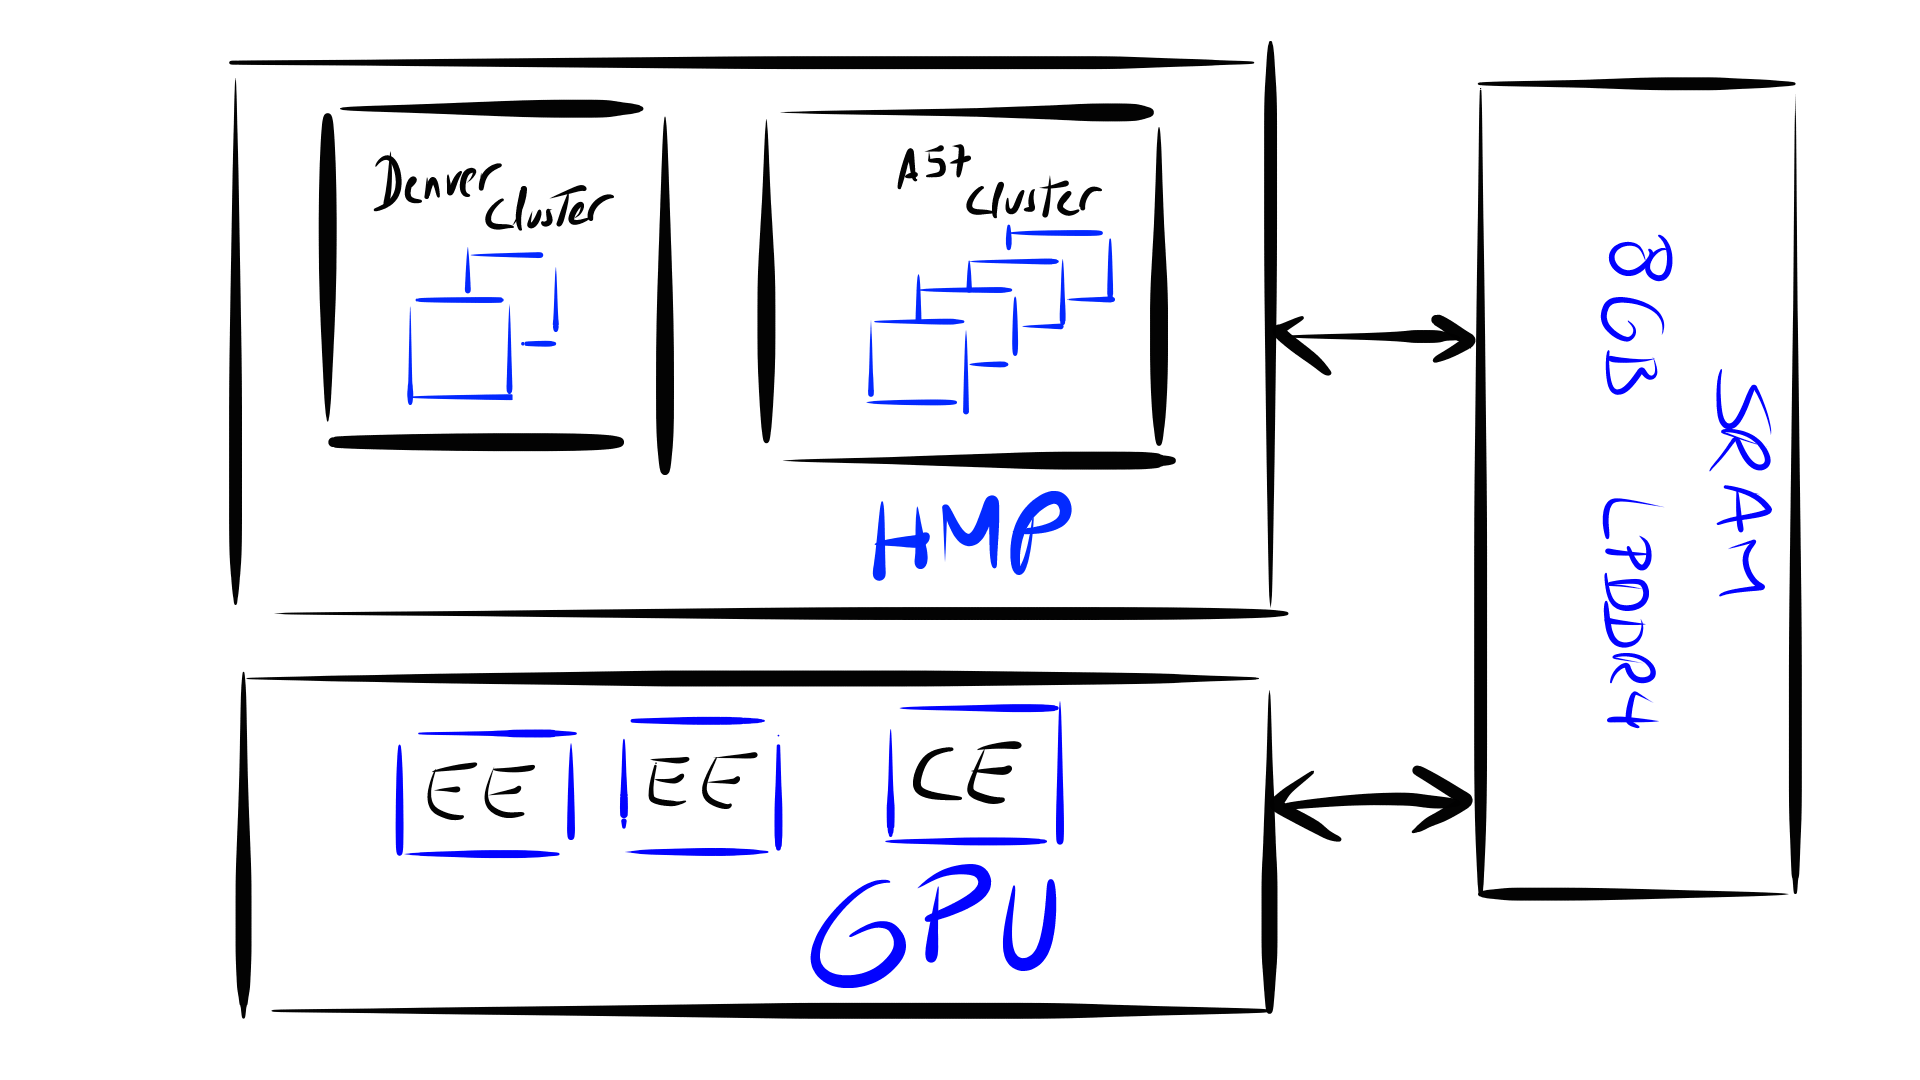
\includegraphics[width=1\textwidth,height=\textheight]{source/figures/overview_arch.png}
\caption{Jetson TX2 Architecture Overview \label{img:overview_arch}}
\end{figure}

Any NVIDIA GPU has two types of engines, \textbf{Copy Engines} (CE) and
\textbf{Execution Engines} (EE). The Jetson TX2 has only one CE and two
EE also known as \textbf{Streaming multiprocessors}. CE is in charge of
data transfers from host to device and viceversa. There is, moreover,
the possibility that EE and CE can run concurrently.

The GPU uses \textbf{streams} to run applications. The number of streams
depends on the GPU resources. An application can run in one or multiple
streams, the GPU scheduler, by default, manages how to application will
be allocated on streams in order to maximize throughput. In Chapter 2,
we will discuss in more detail how the TX2 GPU scheduler behave in case
of multiple applications.

\hypertarget{jetson-tx2-amalthea-model}{%
\section{Jetson TX2 Amalthea Model}\label{jetson-tx2-amalthea-model}}

AMALTHEA is a platform for engineering multi- and many-core embedded
systems. This platform enables the creation and management of complex
tool chains including simulation and validation {[}9{]}. In the context
of WATERS Challenge 2019, Bosch offers an AMALTHEA model of the Jetson
TX2. In this model, a CPU runnable will read data from memory, execute
some computation (Ticks) and write back data into memory as shown in
Figure \ref{img:amalthea01}.

\begin{figure}
\centering
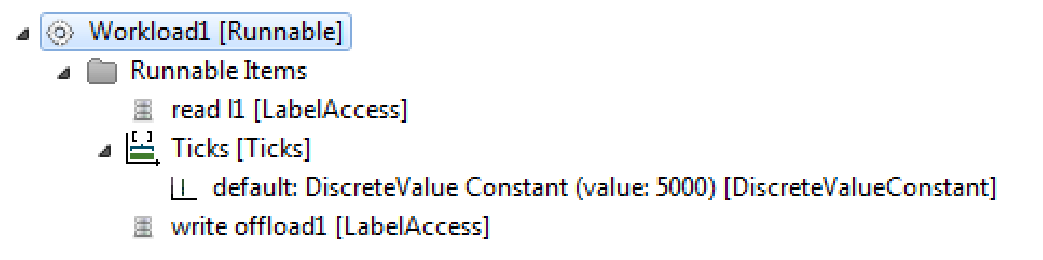
\includegraphics{source/figures/amalthea-01.png}
\caption{Runnable example for a CPU {[}6{]} \label{img:amalthea01}}
\end{figure}

In the case of GPU modeling, the runnable will follow the same pattern
as in the CPU case: read, execution, write back. However, the reading
operation is actually to copy memory from host to device, thus it is
modeled as \emph{memory reading from host} and then as \emph{memory
writing to device}. On the other hand, the writing back operation
requires to copy memory from device to host, therefore it is modeled as
\emph{memory reading from device} and then as \emph{memory writing to
host} as shown in Figure \ref{img:amalthea02}.

\begin{figure}
\centering
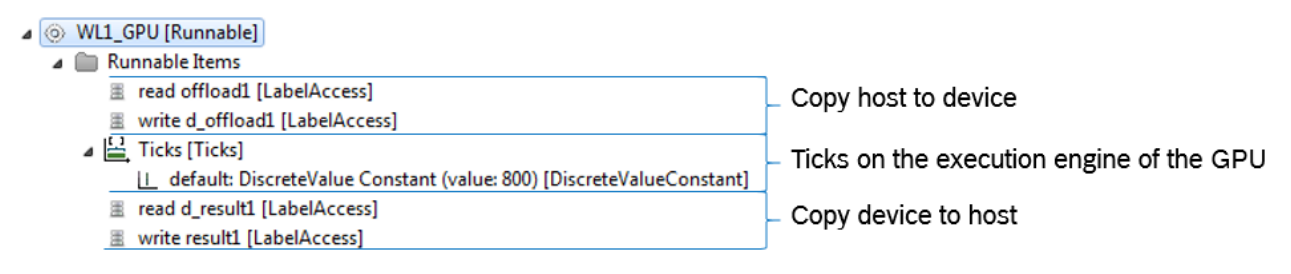
\includegraphics{source/figures/amalthea-02.png}
\caption{Runnable example for a GPU {[}6{]} \label{img:amalthea02}}
\end{figure}

\hypertarget{cuda-and-jetson-tx2}{%
\chapter{CUDA and Jetson TX2}\label{cuda-and-jetson-tx2}}

In this chapter\ldots blablabla

\hypertarget{nvidia-gpu-software-model}{%
\section{NVIDIA GPU Software Model}\label{nvidia-gpu-software-model}}

Now a days computer applications run on heterogeneous hardware and GPUs
are important in order to achieve high performance computing. Since 2006
running software on NVIDIA GPUs are known as a \emph{CUDA application}
{[}10{]}. A CUDA application will run concurrently multiple instances of
special functions called \textbf{kernels}.Each instance runs on a
\textbf{thread}. Moreover, these threads are arranged in
\textbf{blocks}, and blocks compose \textbf{grids} as shown in Figure
\ref{img:sw_model_grids}.

\begin{figure}
\centering
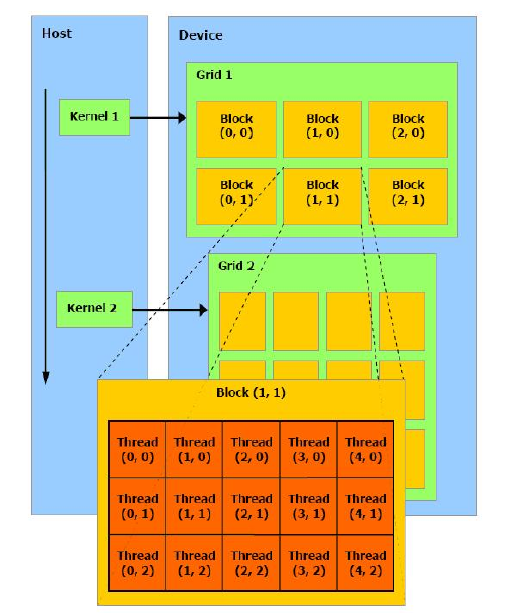
\includegraphics[width=0.6\textwidth,height=\textheight]{source/figures/sw_model_grids.png}
\caption{Organisation of grids, blocks, threads, and kernels {[}11{]}.
\label{img:sw_model_grids}}
\end{figure}

It's logical to think that there is also a hierarchical memory
structure. Threads, blocks and grids have access to different memory
spaces as ilustrated in Figure \ref{img:sw_model_memory}. The types of
memory are summarized in Table \ref{tab:memory_hierarchy}.

\newpage

\begin{longtable}[]{@{}llll@{}}
\caption{Types of memories in a GPU
\label{tab:memory_hierarchy}}\tabularnewline
\toprule
\begin{minipage}[b]{0.13\columnwidth}\raggedright
Memory\strut
\end{minipage} & \begin{minipage}[b]{0.53\columnwidth}\raggedright
Main Characteristics\strut
\end{minipage} & \begin{minipage}[b]{0.09\columnwidth}\raggedright
Scope\strut
\end{minipage} & \begin{minipage}[b]{0.13\columnwidth}\raggedright
Lifetime\strut
\end{minipage}\tabularnewline
\midrule
\endfirsthead
\toprule
\begin{minipage}[b]{0.13\columnwidth}\raggedright
Memory\strut
\end{minipage} & \begin{minipage}[b]{0.53\columnwidth}\raggedright
Main Characteristics\strut
\end{minipage} & \begin{minipage}[b]{0.09\columnwidth}\raggedright
Scope\strut
\end{minipage} & \begin{minipage}[b]{0.13\columnwidth}\raggedright
Lifetime\strut
\end{minipage}\tabularnewline
\midrule
\endhead
\begin{minipage}[t]{0.13\columnwidth}\raggedright
Global\strut
\end{minipage} & \begin{minipage}[t]{0.53\columnwidth}\raggedright
R/W, Slow and big\strut
\end{minipage} & \begin{minipage}[t]{0.09\columnwidth}\raggedright
Grid\strut
\end{minipage} & \begin{minipage}[t]{0.13\columnwidth}\raggedright
Application\strut
\end{minipage}\tabularnewline
\begin{minipage}[t]{0.13\columnwidth}\raggedright
Texture\strut
\end{minipage} & \begin{minipage}[t]{0.53\columnwidth}\raggedright
ROM, Fast, Optimized for 2D/3D access\strut
\end{minipage} & \begin{minipage}[t]{0.09\columnwidth}\raggedright
Grid\strut
\end{minipage} & \begin{minipage}[t]{0.13\columnwidth}\raggedright
Application\strut
\end{minipage}\tabularnewline
\begin{minipage}[t]{0.13\columnwidth}\raggedright
Constant\strut
\end{minipage} & \begin{minipage}[t]{0.53\columnwidth}\raggedright
ROM, Fast, Constants and kernel parameters\strut
\end{minipage} & \begin{minipage}[t]{0.09\columnwidth}\raggedright
Grid\strut
\end{minipage} & \begin{minipage}[t]{0.13\columnwidth}\raggedright
Application\strut
\end{minipage}\tabularnewline
\begin{minipage}[t]{0.13\columnwidth}\raggedright
Shared\strut
\end{minipage} & \begin{minipage}[t]{0.53\columnwidth}\raggedright
R/W, Fast, it's on-chip\strut
\end{minipage} & \begin{minipage}[t]{0.09\columnwidth}\raggedright
Block\strut
\end{minipage} & \begin{minipage}[t]{0.13\columnwidth}\raggedright
Block\strut
\end{minipage}\tabularnewline
\begin{minipage}[t]{0.13\columnwidth}\raggedright
Local\strut
\end{minipage} & \begin{minipage}[t]{0.53\columnwidth}\raggedright
R/W, Slow as global, when registers are full\strut
\end{minipage} & \begin{minipage}[t]{0.09\columnwidth}\raggedright
Thread\strut
\end{minipage} & \begin{minipage}[t]{0.13\columnwidth}\raggedright
Thread\strut
\end{minipage}\tabularnewline
\begin{minipage}[t]{0.13\columnwidth}\raggedright
Registers\strut
\end{minipage} & \begin{minipage}[t]{0.53\columnwidth}\raggedright
R/W, Fast\strut
\end{minipage} & \begin{minipage}[t]{0.09\columnwidth}\raggedright
Thread\strut
\end{minipage} & \begin{minipage}[t]{0.13\columnwidth}\raggedright
Thread\strut
\end{minipage}\tabularnewline
\bottomrule
\end{longtable}

\begin{figure}
\centering
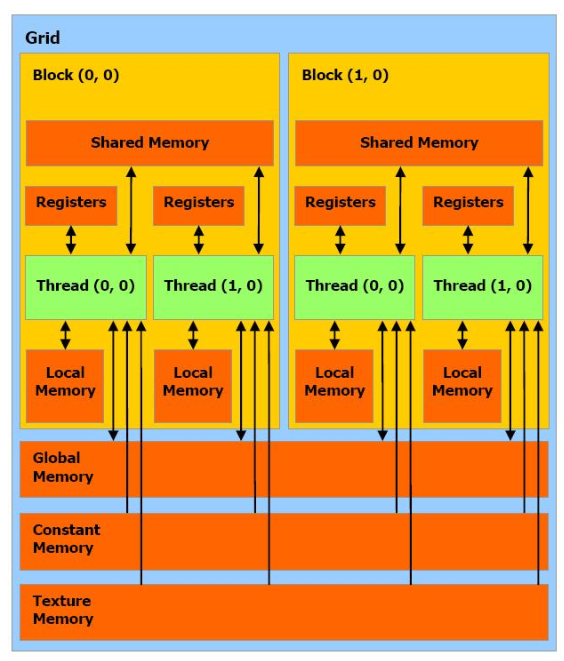
\includegraphics[width=0.6\textwidth,height=\textheight]{source/figures/sw_model_memory.png}
\caption{Memory hierarchy {[}11{]}. \label{img:sw_model_memory}}
\end{figure}

In summary, CUDA application solve problems that were modeled based on
\emph{divide and conquer} principle. Moreover, CUDA software model not
only allow users to achieve high computational performance, but also
CUDA application are highly scalable.

\hypertarget{nvidia-gpu-hardware-model}{%
\section{NVIDIA GPU Hardware Model}\label{nvidia-gpu-hardware-model}}

The CUDA architecture is based on \textbf{Streaming Multiprocessors}
(SM) which perform the actual computation. Each SM has it own control
units, registers, execution pipelines and local memories, but they also
have access to global memory as ilustrated in Figure
\ref{img:sm_memory}. A \textbf{stream} is a queue of CUDA operations,
memory copy and kernel launch. We will talk more about streams in
following sections.

\begin{figure}
\centering
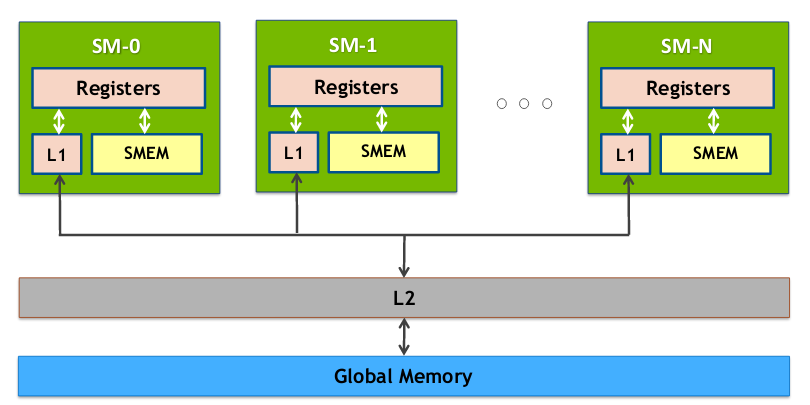
\includegraphics[width=0.6\textwidth,height=\textheight]{source/figures/sm_memory.png}
\caption{Memory hierarchy \label{img:sm_memory}}
\end{figure}

When a kernel grid is launch blocks are enumerated and assigend to the
SMs. Once the blocks are assigned, threads are managed in \textbf{wraps}
by the \textbf{wrap scheduler}. A wraps is a group of 32 threads that
run in parallel. Thus, it's highly recommendable to use block sizes of
size \(32N, N \in \mathbb{N}\), otherwise there would be ``inactive''
threads. A example is shown in Figure \ref{img:inactive_thread}, where
there is a block of 140 threads but since the wrap scheduler works with
wraps, 20 threads are wasted and no other block can make use of them.

\begin{figure}
\centering
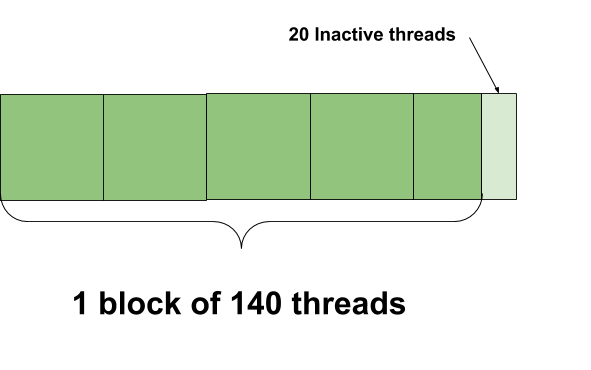
\includegraphics[width=0.6\textwidth,height=\textheight]{source/figures/inactive_thread.png}
\caption{Inactive threads \label{img:inactive_thread}}
\end{figure}

The amount of threads and blocks that can run concurrently per SM
depends on the number of 32-bit registers and shared memory within SM,
as well as the CUDA computing capability of the GPU. Information related
to maximum amount of blocks or threads, as well as the computing
capability of the GPU can be display executing \texttt{deviceQuery}
tool. Some information about Jetson TX2 is presented below:

\begin{Shaded}
\begin{Highlighting}[]
\ExtensionTok{CUDA}\NormalTok{ Device Query (Runtime API) }\ExtensionTok{version}\NormalTok{ (CUDART static linking)}
\ExtensionTok{Detected}\NormalTok{ 1 CUDA Capable device(s)}
\ExtensionTok{Device}\NormalTok{ 0: }\StringTok{"NVIDIA Tegra X2"}
  \ExtensionTok{CUDA}\NormalTok{ Driver Version / Runtime Version     9.0 / 9.0}
  \ExtensionTok{CUDA}\NormalTok{ Capability:                          6.2}
  \ExtensionTok{Total}\NormalTok{ amount of global memory:            7850 MBytes }
  \KeywordTok{(} \ExtensionTok{2}\KeywordTok{)} \ExtensionTok{SM}\NormalTok{, (128) }\ExtensionTok{CUDA}\NormalTok{ Cores/SM:             256 CUDA Cores}
  \ExtensionTok{L2}\NormalTok{ Cache Size:                            524288 bytes}
  \ExtensionTok{Total}\NormalTok{ amount of shared memory per block:  49152 bytes}
  \ExtensionTok{Total}\NormalTok{ number of registers per block:      32768}
  \ExtensionTok{Warp}\NormalTok{ size:                                32}
  \ExtensionTok{Max.}\NormalTok{ number of threads per SM:            2048}
  \ExtensionTok{Max.}\NormalTok{ number of threads per block:         1024}
  \ExtensionTok{Max}\NormalTok{ dim. size of a thread block (x,y,z)}\BuiltInTok{:}\NormalTok{  (1024, 1024, 64)}
  \ExtensionTok{Max}\NormalTok{ dim. size of a grid size    (x,y,z)}\BuiltInTok{:}\NormalTok{  (2\^{}31{-}1, 65535, 65535)}
\end{Highlighting}
\end{Shaded}

\hypertarget{nvidia-jetson-tx2s-gpu-scheduler}{%
\section{NVIDIA Jetson TX2's GPU
Scheduler}\label{nvidia-jetson-tx2s-gpu-scheduler}}

It's common to use several kernels in an application. In order to reduce
computation time and maximaze GPU utilization, it's desire to run
multiple kernels in parallel. CUDA uses streams to achieve this goal. As
mentioned before, a stream is a queue of CUDA operations, memory copy
and kernel launch. Thus, it is possible either to launch multiple
kernels within one streams or multiple kernels on multiple streams.
Operations within the same stream are managed in FIFO (First In First
Out) fashion, thus, we will also use the term \textbf{stream queue} when
we talk about FIFO queues within a stream. The Jeston TX2's GPU assigns
resources to streams using its internal scheduler.

Predictability is an important characteristic of safety-critical
systems. It requires both functional and timing correctness. However, a
detailed information about the Jetson TX2's GPU scheduler behaviour is
not publicly available. Without such details, it is imposible to analyze
timing constrains. Nevertheless, there are some efforts {[}12{]},
{[}13{]} and {[}14{]} aimed at revealing these details through black-box
experimentation.

NVIDIA GPU scheduling policies depend on whether the GPU workloads are
launched by a CPU executing OS threads or OS processes. We will focus on
the first case, because GPU computations launched by OS processes have
more unpredictable behaviours, as stated in {[}12{]} and {[}13{]}. In
this section, we will present GPU scheduling policies devired by
{[}12{]} and use them in an example to clarify their use.

Let's start by defining some terms. When one block of a kernel has been
scheduled for execution on a SM it's said that the block was
\textbf{assigned}. Moreover, it's said a kernel was \textbf{dispatched}
as soon as one of its blocks were assigned, and \textbf{fully
dispatched} once all its blocks were assigned. The same applies to copy
operations and CE.\\
There are, in addition, FIFO CE queues used to schedule copy operations,
and FIFO EE queues used to schedule kernel launches. Stream queues feed
CE and EE queues. Bellow we will present the rules that determine
scheduler and queues behaviours.

\begin{itemize}
\tightlist
\item
  \textbf{General Scheduling Rules}:

  \begin{itemize}
  \tightlist
  \item
    \textbf{G1} A copy operation or kernel is enqueued on the stream
    queue for its stream when the associated CUDA API function (memory
    transfer or kernel launch) is invoked.
  \item
    \textbf{G2} A kernel is enqueued on the EE queue when it reaches the
    head of its stream queue.
  \item
    \textbf{G3} A kernel at the head of the EE queue is dequeued from
    that queue once it becomes fully dispatched.
  \item
    \textbf{G4} A kernel is dequeued from its stream queue once all of
    its blocks complete execution.
  \end{itemize}
\item
  \textbf{Non-preemptive execution}:

  \begin{itemize}
  \tightlist
  \item
    \textbf{X1} Only blocks of the kernel at the head of the EE queue
    are eligible to be assigned.
  \end{itemize}
\item
  \textbf{Rules governing thread resources}:

  \begin{itemize}
  \tightlist
  \item
    \textbf{R1} A block of the kernel at the head of the EE queue is
    eligible to be assigned only if its resource constraints are met.
  \item
    \textbf{R2} A block of the kernel at the head of the EE queue is
    eligible to be assigned only if there are sufficient thread
    resources available on some SM.
  \end{itemize}
\item
  \textbf{Rules governing shared-memory resources}:

  \begin{itemize}
  \tightlist
  \item
    \textbf{R3} A block of the kernel at the head of the EE queue is
    eligible to be assigned only if there are sufficient shared-memory
    resources available on some SM.
  \end{itemize}
\item
  \textbf{Copy operations}:

  \begin{itemize}
  \tightlist
  \item
    \textbf{C1} A copy operation is enqueued on the CE queue when it
    reaches the head of its stream queue.
  \item
    \textbf{C2} A copy operation at the head of the CE queue is eligible
    to be assigned to the CE.
  \item
    \textbf{C3} A copy operation at the head of the CE queue is dequeued
    from the CE queue once the copy is
  \item
    \textbf{C4} A copy operation is dequeued from its stream queue once
    the CE has completed the copy.
  \end{itemize}
\item
  \textbf{Streams with priorities}:

  \begin{itemize}
  \tightlist
  \item
    \textbf{A1} A kernel can only be enqueued on the EE queue matching
    the priority of its stream.
  \item
    \textbf{A2} A block of a kernel at the head of any EE queue is
    eligible to be assigned only if all higher-priority EE queues
    (priority-high over priority-low) are empty.
  \end{itemize}
\end{itemize}

Authors in {[}12{]} mentioned that rules related to \textbf{registry
resources} are expected to have exactly the same impact as threads and
shared-memory rules.

\begin{figure}
\centering
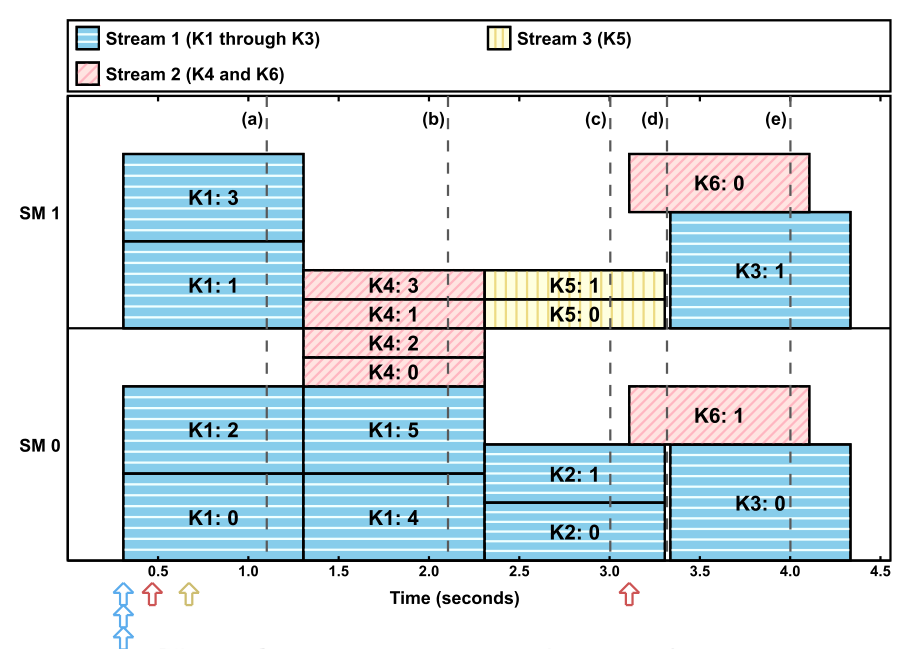
\includegraphics[width=0.6\textwidth,height=\textheight]{source/figures/scheduler_blocks.png}
\caption{Basic GPU scheduling experiment {[}12{]}
\label{img:scheduler_blocks}}
\end{figure}

\begin{figure}
\centering
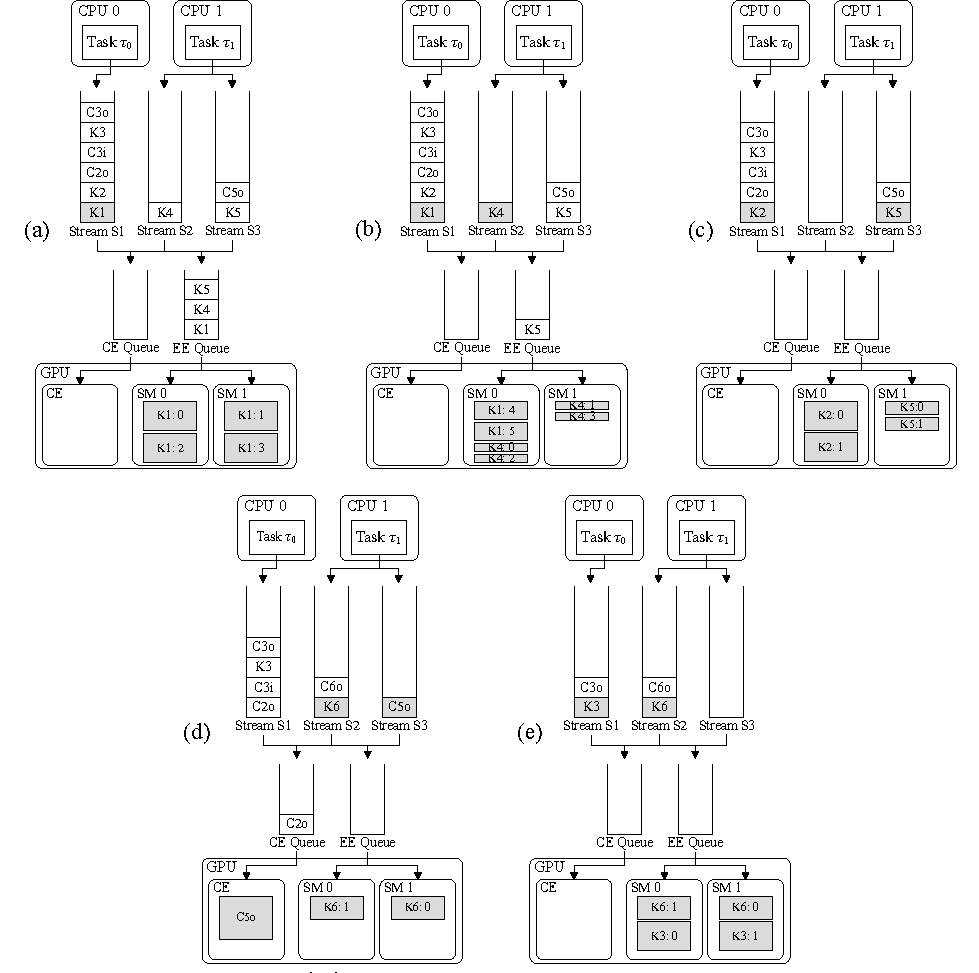
\includegraphics[width=1\textwidth,height=\textheight]{source/figures/scheduler_queues.png}
\caption{Detailed state information at various time points in Fig.
\ref{img:scheduler_blocks} {[}12{]} .\label{img:scheduler_queues}}
\end{figure}

\begin{table}[hbtp]
\small
\begin{tabularx}{\linewidth}{|X|X|X|X|X|}
    \hline
Rules & (a) t=1.0s & (b) t=2.1s & (c) t=3.0s & (d) t=3.4s \\ \hline
G1 & All Kernels except for K6 were enqueued on their streams. K6 is launched at t = 3.2s & K6 operations are not yet enqueued on  S2. Same reason as in (a). & Same situation as in (b). & K6 operations were enqueued at t=3.2s on S2. \\ \hline
G2 & K1, K4, K5 were at the head of their streams. They were enqueued on EE queue. & There are not new kernel at the head of stream queues. & K2 was enqueued on EE queue. & K6 kernel was enqueued on EE, because it was at the head of S2. \\ \hline
G3 & No kernels fullfill this rule. & K1, K4 have dispatched all their blocks. K5 is the only one on the EE queue. & K5, K2 were dequeued from EE queue, because all their blocks were dispatched.  & K6 was fully dispatched, thus was dequeued from EE queue. \\ \hline
G4 & No kernels fullfill this rule. K1 still has running blocks. & K1, K4 still have running blocks. Thus they cannot be dequeued from their stream queues. & K1, K4 were dequeued from their stream queues, because all their blocks finished execution. K2, K5 still have running blocks, they cannot be dequeued from stream queues. & K6 still have running blocks. Thus cannot be yet dequeued from S2. \\ \hline
\end{tabularx}
\label{tab:scheduler_rules1}
\caption{Detailed state information at various time points in Fig.}
\end{table}


\begin{table}[hbtp]
    \small
\begin{tabularx}{\linewidth}{|X|X|X|X|X|}
    \hline
Rules & (a) t=1.0s & (b) t=2.1s & (c) t=3.0s & (d) t=3.4s \\ \hline
X1 & K4 cannot be launched because of this rule, even when there are enough resources (512 threads) & K4 was the next kernel on the EE queue. It was launch because K1 already dispatched it's remaining blocks. & K5 blocks became eligible then dispatched. After that K2 blocks became eligible and then dispatched. & K6 blocks became eligible, because K6 was at the head of EE queue. \\ \hline
R1 & Applies only to K1. & K5 is eligible, but check R3 & K5 became eligible. K2 became eligible after K5. & There were enough resources for K6. \\ \hline
R2 & Applies only to K1. & K5 is eligible, but check R3 & There were enough thread resources for K2 and K5 (1024 threads in SM0, and 1536 threads in SM1). & There were enough thread resources in each SM for K6 (free 512 threads per SM , each K6 block needed 512 threads). \\ \hline
R3 & Applies only to K1. & There is not enough shared memory to launch K5.  Each K5 block requires 32KB (64KB in total), but K4 blocks are consuming the whole shared memory available per SM (64KB). & There were enough shared memory for K2 and K5 (64KB in each SM). & K6 blocks required no memory shared.  \\ \hline
\end{tabularx}
\label{tab:scheduler_rules2}
\caption{Detailed state information at various time points in Fig.}
\end{table}


\begin{table}[hbtp]
\small
\begin{tabularx}{\linewidth}{|X|X|X|X|X|}
    \hline
Rules & (a) t=1.0s & (b) t=2.1s & (c) t=3.0s & (d) t=3.4s \\ \hline
C1 & No copy operations at the head of streams. & No copy operations at the head of streams. & No copy operations at the head of streams. & C5o, C2o were enqueued on CE queue. \\ \hline
C2 & No available copy operations. & No available copy operations. & No available copy operations. & C5o was assigned to CE. \\ \hline
C3 & No available copy operations. & No available copy operations. & No available copy operations. & C5o was dequeued from CE. \\ \hline
C4 & No copy operations at the head of streams. & No copy operations at the head of streams. & No copy operations at the head of streams. & C5o is still copying. Thus it cannot be dequeued from S3. \\ \hline
\end{tabularx}
\label{tab:scheduler_rules3}
\caption{Detailed state information at various time points in Fig.}
\end{table}

\newpage

\hypertarget{first-research-study-with-code}{%
\chapter{First research study, with
code}\label{first-research-study-with-code}}

\hypertarget{introduction-1}{%
\section{Introduction}\label{introduction-1}}

This is the introduction. Nam mollis congue tortor, sit amet convallis
tortor mollis eget. Fusce viverra ut magna eu sagittis. Vestibulum at
ultrices sapien, at elementum urna. Nam a blandit leo, non lobortis
quam. Aliquam feugiat turpis vitae tincidunt ultricies. Mauris
ullamcorper pellentesque nisl, vel molestie lorem viverra at.

\hypertarget{method}{%
\section{Method}\label{method}}

Suspendisse iaculis in lacus ut dignissim. Cras dignissim dictum
eleifend. Suspendisse potenti. Suspendisse et nisi suscipit, vestibulum
est at, maximus sapien. Sed ut diam tortor.

\hypertarget{subsection-1-with-example-code-block}{%
\subsection{Subsection 1 with example code
block}\label{subsection-1-with-example-code-block}}

This is the first part of the methodology. Cras porta dui a dolor
tincidunt placerat. Cras scelerisque sem et malesuada vestibulum.
Vivamus faucibus ligula ac sodales consectetur. Aliquam vel tristique
nisl. Aliquam erat volutpat. Pellentesque iaculis enim sit amet posuere
facilisis. Integer egestas quam sit amet nunc maximus, id bibendum ex
blandit.

For syntax highlighting in code blocks, add three ```'' characters
before and after a code block:

\begin{Shaded}
\begin{Highlighting}[]
\NormalTok{mood }\OperatorTok{=} \StringTok{\textquotesingle{}happy\textquotesingle{}}
\ControlFlowTok{if}\NormalTok{ mood }\OperatorTok{==} \StringTok{\textquotesingle{}happy\textquotesingle{}}\NormalTok{:}
    \BuiltInTok{print}\NormalTok{(}\StringTok{"I am a happy robot"}\NormalTok{)}
\end{Highlighting}
\end{Shaded}

Alternatively, you can also use LaTeX to create a code block as shown in
the Java example below:

\lstinputlisting[style=javaCodeStyle, caption=Main.java]{source/code/HelloWorld.java}

If you use \texttt{javaCodeStyle} as defined in the
\texttt{preamble.tex}, it is best to keep the maximum line length in the
source code at 80 characters.

\hypertarget{subsection-2}{%
\subsection{Subsection 2}\label{subsection-2}}

This is the second part of the methodology. Proin tincidunt odio non sem
mollis tristique. Fusce pharetra accumsan volutpat. In nec mauris vel
orci rutrum dapibus nec ac nibh. Praesent malesuada sagittis nulla, eget
commodo mauris ultricies eget. Suspendisse iaculis finibus ligula.

\hypertarget{results}{%
\section{Results}\label{results}}

These are the results. Ut accumsan tempus aliquam. Sed massa ex, egestas
non libero id, imperdiet scelerisque augue. Duis rutrum ultrices arcu et
ultricies. Proin vel elit eu magna mattis vehicula. Sed ex erat,
fringilla vel feugiat ut, fringilla non diam.

\hypertarget{discussion}{%
\section{Discussion}\label{discussion}}

This is the discussion. Duis ultrices tempor sem vitae convallis.
Pellentesque lobortis risus ac nisi varius bibendum. Phasellus volutpat
aliquam varius. Mauris vitae neque quis libero volutpat finibus. Nunc
diam metus, imperdiet vitae leo sed, varius posuere orci.

\hypertarget{conclusion}{%
\section{Conclusion}\label{conclusion}}

This is the conclusion to the chapter. Praesent bibendum urna orci, a
venenatis tellus venenatis at. Etiam ornare, est sed lacinia elementum,
lectus diam tempor leo, sit amet elementum ex elit id ex. Ut ac viverra
turpis. Quisque in nisl auctor, ornare dui ac, consequat tellus.

\hypertarget{research-containing-a-figure}{%
\chapter{Research containing a
figure}\label{research-containing-a-figure}}

\hypertarget{introduction-2}{%
\section{Introduction}\label{introduction-2}}

This is the introduction. Sed vulputate tortor at nisl blandit interdum.
Cras sagittis massa ex, quis eleifend purus condimentum congue. Maecenas
tristique, justo vitae efficitur mollis, mi nulla varius elit, in
consequat ligula nulla ut augue. Phasellus diam sapien, placerat sit
amet tempor non, lobortis tempus ante.

\hypertarget{method-1}{%
\section{Method}\label{method-1}}

Donec imperdiet, lectus vestibulum sagittis tempus, turpis dolor euismod
justo, vel tempus neque libero sit amet tortor. Nam cursus commodo
tincidunt.

\hypertarget{subsection-1}{%
\subsection{Subsection 1}\label{subsection-1}}

This is the first part of the methodology. Duis tempor sapien sed tellus
ultrices blandit. Sed porta mauris tortor, eu vulputate arcu dapibus ac.
Curabitur sodales at felis efficitur sollicitudin. Quisque at neque
sollicitudin, mollis arcu vitae, faucibus tellus.

\hypertarget{subsection-2-1}{%
\subsection{Subsection 2}\label{subsection-2-1}}

This is the second part of the methodology. Sed ut ipsum ultrices,
interdum ipsum vel, lobortis diam. Curabitur sit amet massa quis tortor
molestie dapibus a at libero. Mauris mollis magna quis ante vulputate
consequat. Integer leo turpis, suscipit ac venenatis pellentesque,
efficitur non sem. Pellentesque eget vulputate turpis. Etiam id nibh at
elit fermentum interdum.

\hypertarget{results-1}{%
\section{Results}\label{results-1}}

These are the results. In vitae odio at libero elementum fermentum vel
iaculis enim. Nullam finibus sapien in congue condimentum. Curabitur et
ligula et ipsum mollis fringilla.

\hypertarget{discussion-1}{%
\section{Discussion}\label{discussion-1}}

Figure \ref{ref_a_figure} shows how to add a figure. Donec ut lacinia
nibh. Nam tincidunt augue et tristique cursus. Vestibulum sagittis odio
nisl, a malesuada turpis blandit quis. Cras ultrices metus tempor
laoreet sodales. Nam molestie ipsum ac imperdiet laoreet. Pellentesque
habitant morbi tristique senectus et netus et malesuada fames ac turpis
egestas.

\begin{figure}
\centering
\includegraphics[width=1\textwidth,height=\textheight]{source/figures/example_figure.pdf}
\caption{RV Calypso is a former British Royal Navy minesweeper converted
into a research vessel for the oceanographic researcher Jacques-Yves
Cousteau. It was equipped with a mobile laboratory for underwater field
research. \label{ref_a_figure}}
\end{figure}

\hypertarget{conclusion-1}{%
\section{Conclusion}\label{conclusion-1}}

This is the conclusion to the chapter. Quisque nec purus a quam
consectetur volutpat. Cum sociis natoque penatibus et magnis dis
parturient montes, nascetur ridiculus mus. In lorem justo, convallis
quis lacinia eget, laoreet eu metus. Fusce blandit tellus tellus.
Curabitur nec cursus odio. Quisque tristique eros nulla, vitae finibus
lorem aliquam quis. Interdum et malesuada fames ac ante ipsum primis in
faucibus.

\hypertarget{research-containing-a-table}{%
\chapter{Research containing a
table}\label{research-containing-a-table}}

\hypertarget{introduction-3}{%
\section{Introduction}\label{introduction-3}}

This is the introduction. Phasellus non purus id mauris aliquam rutrum
vitae quis tellus. Maecenas rhoncus ligula nulla, fringilla placerat mi
consectetur eu. Aenean nec metus ac est ornare posuere. Nunc ipsum
lacus, gravida commodo turpis quis, rutrum eleifend erat. Pellentesque
id lorem eget ante porta tincidunt nec nec tellus.

\hypertarget{method-2}{%
\section{Method}\label{method-2}}

Vivamus consectetur, velit in congue lobortis, massa massa lacinia urna,
sollicitudin semper ipsum augue quis tortor. Donec quis nisl at arcu
volutpat ultrices. Maecenas ex nibh, consequat ac blandit sit amet,
molestie in odio. Morbi finibus libero et nisl dignissim, at ultricies
ligula pulvinar.

\hypertarget{subsection-1-1}{%
\subsection{Subsection 1}\label{subsection-1-1}}

This is the first part of the methodology. Integer leo erat, commodo in
lacus vel, egestas varius elit. Nulla eget magna quam. Nullam
sollicitudin dolor ut ipsum varius tincidunt. Duis dignissim massa in
ipsum accumsan imperdiet. Maecenas suscipit sapien sed dui pharetra
blandit. Morbi fermentum est vel quam pretium maximus.

\hypertarget{subsection-2-2}{%
\subsection{Subsection 2}\label{subsection-2-2}}

This is the second part of the methodology. Nullam accumsan condimentum
eros eu volutpat. Maecenas quis ligula tempor, interdum ante sit amet,
aliquet sem. Fusce tellus massa, blandit id tempus at, cursus in tortor.
Nunc nec volutpat ante. Phasellus dignissim ut lectus quis porta. Lorem
ipsum dolor sit amet, consectetur adipiscing elit.

\hypertarget{results-2}{%
\section{Results}\label{results-2}}

Table \ref{ref_a_table} shows us how to add a table. Integer tincidunt
sed nisl eget pellentesque. Mauris eleifend, nisl non lobortis
fringilla, sapien eros aliquet orci, vitae pretium massa neque eu
turpis. Pellentesque tincidunt aliquet volutpat. Ut ornare dui id ex
sodales laoreet.

\newpage

\begin{longtable}[]{@{}lll@{}}
\caption{This is the table caption. Suspendisse blandit dolor sed tellus
venenatis, venenatis fringilla turpis pretium.
\label{ref_a_table}}\tabularnewline
\toprule
\begin{minipage}[b]{0.25\columnwidth}\raggedright
Column 1\strut
\end{minipage} & \begin{minipage}[b]{0.30\columnwidth}\raggedright
Column 2\strut
\end{minipage} & \begin{minipage}[b]{0.25\columnwidth}\raggedright
Column 3\strut
\end{minipage}\tabularnewline
\midrule
\endfirsthead
\toprule
\begin{minipage}[b]{0.25\columnwidth}\raggedright
Column 1\strut
\end{minipage} & \begin{minipage}[b]{0.30\columnwidth}\raggedright
Column 2\strut
\end{minipage} & \begin{minipage}[b]{0.25\columnwidth}\raggedright
Column 3\strut
\end{minipage}\tabularnewline
\midrule
\endhead
\begin{minipage}[t]{0.25\columnwidth}\raggedright
Row 1\strut
\end{minipage} & \begin{minipage}[t]{0.30\columnwidth}\raggedright
0.1\strut
\end{minipage} & \begin{minipage}[t]{0.25\columnwidth}\raggedright
0.2\strut
\end{minipage}\tabularnewline
\begin{minipage}[t]{0.25\columnwidth}\raggedright
Row 2\strut
\end{minipage} & \begin{minipage}[t]{0.30\columnwidth}\raggedright
0.3\strut
\end{minipage} & \begin{minipage}[t]{0.25\columnwidth}\raggedright
0.3\strut
\end{minipage}\tabularnewline
\begin{minipage}[t]{0.25\columnwidth}\raggedright
Row 3\strut
\end{minipage} & \begin{minipage}[t]{0.30\columnwidth}\raggedright
0.4\strut
\end{minipage} & \begin{minipage}[t]{0.25\columnwidth}\raggedright
0.4\strut
\end{minipage}\tabularnewline
\begin{minipage}[t]{0.25\columnwidth}\raggedright
Row 4\strut
\end{minipage} & \begin{minipage}[t]{0.30\columnwidth}\raggedright
0.5\strut
\end{minipage} & \begin{minipage}[t]{0.25\columnwidth}\raggedright
0.6\strut
\end{minipage}\tabularnewline
\bottomrule
\end{longtable}

\hypertarget{discussion-2}{%
\section{Discussion}\label{discussion-2}}

This is the discussion. Etiam sit amet mi eros. Donec vel nisi sed purus
gravida fermentum at quis odio. Vestibulum quis nisl sit amet justo
maximus molestie. Maecenas vitae arcu erat. Nulla facilisi. Nam pretium
mauris eu enim porttitor, a mattis velit dictum. Nulla sit amet ligula
non mauris volutpat fermentum quis vitae sapien.

\hypertarget{conclusion-2}{%
\section{Conclusion}\label{conclusion-2}}

This is the conclusion to the chapter. Nullam porta tortor id vehicula
interdum. Quisque pharetra, neque ut accumsan suscipit, orci orci
commodo tortor, ac finibus est turpis eget justo. Cras sodales nibh nec
mauris laoreet iaculis. Morbi volutpat orci felis, id condimentum nulla
suscipit eu. Fusce in turpis quis ligula tempus scelerisque eget quis
odio. Vestibulum et dolor id erat lobortis ullamcorper quis at sem.

\hypertarget{final-research-study}{%
\chapter{Final research study}\label{final-research-study}}

\hypertarget{introduction-4}{%
\section{Introduction}\label{introduction-4}}

This is the introduction. Nunc lorem odio, laoreet eu turpis at,
condimentum sagittis diam. Phasellus metus ligula, auctor ac nunc vel,
molestie mattis libero. Praesent id posuere ex, vel efficitur nibh.
Quisque vestibulum accumsan lacus vitae mattis.

\hypertarget{method-3}{%
\section{Method}\label{method-3}}

In tincidunt viverra dolor, ac pharetra tellus faucibus eget.
Pellentesque tempor a enim nec venenatis. Morbi blandit magna imperdiet
posuere auctor. Maecenas in maximus est.

\hypertarget{subsection-1-2}{%
\subsection{Subsection 1}\label{subsection-1-2}}

This is the first part of the methodology. Praesent mollis sem diam, sit
amet tristique lacus vulputate quis. Vivamus rhoncus est rhoncus tellus
lacinia, a interdum sem egestas. Curabitur quis urna vel quam blandit
semper vitae a leo. Nam vel lectus lectus.

\hypertarget{subsection-2-3}{%
\subsection{Subsection 2}\label{subsection-2-3}}

This is the second part of the methodology. Aenean vel pretium tortor.
Aliquam erat volutpat. Quisque quis lobortis mi. Nulla turpis leo,
ultrices nec nulla non, ullamcorper laoreet risus.

\hypertarget{results-3}{%
\section{Results}\label{results-3}}

These are the results. Curabitur vulputate nisl non ante tincidunt
tempor. Aenean porta nisi quam, sed ornare urna congue sed. Curabitur in
sapien justo. Quisque pulvinar ullamcorper metus, eu varius mauris
pellentesque et. In hac habitasse platea dictumst. Pellentesque nec
porttitor libero. Duis et magna a massa lacinia cursus.

\hypertarget{discussion-3}{%
\section{Discussion}\label{discussion-3}}

This is the discussion. Curabitur gravida nisl id gravida congue. Duis
est nisi, sagittis eget accumsan ullamcorper, semper quis turpis. Mauris
ultricies diam metus, sollicitudin ultricies turpis lobortis vitae. Ut
egestas vehicula enim, porta molestie neque consectetur placerat.
Integer iaculis sapien dolor, non porta nibh condimentum ut.

\hypertarget{conclusion-3}{%
\section{Conclusion}\label{conclusion-3}}

This is the conclusion to the chapter. Nulla sed condimentum lectus.
Duis sed tempor erat, at cursus lacus. Nam vitae tempus arcu, id
vestibulum sapien. Cum sociis natoque penatibus et magnis dis parturient
montes, nascetur ridiculus mus.

\hypertarget{conclusion-4}{%
\chapter{Conclusion}\label{conclusion-4}}

\hypertarget{thesis-summary}{%
\section{Thesis summary}\label{thesis-summary}}

In summary, pellentesque habitant morbi tristique senectus et netus et
malesuada fames ac turpis egestas. Nunc eleifend, ex a luctus porttitor,
felis ex suscipit tellus, ut sollicitudin sapien purus in libero. Nulla
blandit eget urna vel tempus. Praesent fringilla dui sapien, sit amet
egestas leo sollicitudin at.

\hypertarget{future-work}{%
\section{Future work}\label{future-work}}

There are several potential directions for extending this thesis. Lorem
ipsum dolor sit amet, consectetur adipiscing elit. Aliquam gravida ipsum
at tempor tincidunt. Aliquam ligula nisl, blandit et dui eu, eleifend
tempus nibh. Nullam eleifend sapien eget ante hendrerit commodo.
Pellentesque pharetra erat sit amet dapibus scelerisque.

Vestibulum suscipit tellus risus, faucibus vulputate orci lobortis eget.
Nunc varius sem nisi. Nunc tempor magna sapien, euismod blandit elit
pharetra sed. In dapibus magna convallis lectus sodales, a consequat sem
euismod. Curabitur in interdum purus. Integer ultrices laoreet aliquet.
Nulla vel dapibus urna. Nunc efficitur erat ac nisi auctor sodales.

\hypertarget{appendix-1-some-extra-stuff}{%
\chapter*{Appendix 1: Some extra
stuff}\label{appendix-1-some-extra-stuff}}
\addcontentsline{toc}{chapter}{Appendix 1: Some extra stuff}

Add appendix 1 here. Vivamus hendrerit rhoncus interdum. Sed ullamcorper
et augue at porta. Suspendisse facilisis imperdiet urna, eu pellentesque
purus suscipit in. Integer dignissim mattis ex aliquam blandit.
Curabitur lobortis quam varius turpis ultrices egestas.

\hypertarget{appendix-2-some-more-extra-stuff}{%
\chapter*{Appendix 2: Some more extra
stuff}\label{appendix-2-some-more-extra-stuff}}
\addcontentsline{toc}{chapter}{Appendix 2: Some more extra stuff}

Add appendix 2 here. Aliquam rhoncus mauris ac neque imperdiet, in
mattis eros aliquam. Etiam sed massa et risus posuere rutrum vel et
mauris. Integer id mauris sed arcu venenatis finibus. Etiam nec
hendrerit purus, sed cursus nunc. Pellentesque ac luctus magna. Aenean
non posuere enim, nec hendrerit lacus. Etiam lacinia facilisis tempor.
Aenean dictum nunc id felis rhoncus aliquam.

\footnotesize

\hypertarget{references}{%
\chapter*{References}\label{references}}
\addcontentsline{toc}{chapter}{References}

\hypertarget{refs}{}
\leavevmode\hypertarget{ref-Hansen2019}{}%
{[}1{]} ``BMW and audi want to separate vehicle hardware from
software.''
\url{https://www.electronicdesign.com/automotive/bmw-and-audi-want-separate-vehicle-hardware-software}.

\leavevmode\hypertarget{ref-Future2019}{}%
{[}2{]} ``End to end architecture.''
\url{https://www.future-mobility-tech.com/en/technology/end-to-end-architecture}.

\leavevmode\hypertarget{ref-Kanajan2006}{}%
{[}3{]} S. Kanajan, H. Zeng, C. Pinello, and A. Sangiovanni-Vincentelli,
``Exploring trade-off's between centralized versus decentralized
automotive architectures using a virtual integration environment,'' in
\emph{Proceedings of the conference on design, automation and test in
europe: Proceedings}, 2006, pp. 548--553.

\leavevmode\hypertarget{ref-Henzinger2008}{}%
{[}4{]} T. A Henzinger, ``Two challenges in embedded systems design:
Predictability and robustness,'' \emph{Philosophical transactions.
Series A, Mathematical, physical, and engineering sciences}, vol. 366,
pp. 3727--36, Nov. 2008.

\leavevmode\hypertarget{ref-Cullmann2010}{}%
{[}5{]} C. Cullmann \emph{et al.}, ``Predictability considerations in
the design of multi-core embedded systems,'' \emph{Ingénieurs de
l'Automobile}, vol. 807, pp. 36--42, Sep. 2010.

\leavevmode\hypertarget{ref-Water2019Url}{}%
{[}6{]} ``WATERS 2019 -- industrial challenge.''
\url{https://www.ecrts.org/waters/waters-industrial-challenge/}.

\leavevmode\hypertarget{ref-TX2Intro2017}{}%
{[}7{]} D. Franklin, ``NVIDIA jetson tx2 delivers twice the intelligence
to the edge.''
\url{https://devblogs.nvidia.com/jetson-tx2-delivers-twice-intelligence-edge/}.

\leavevmode\hypertarget{ref-TX2Datasheet2014}{}%
{[}8{]} \emph{NVIDIA jetson tx2 system-on-module}. NVIDIA Corporation,
2014.

\leavevmode\hypertarget{ref-Amalthea2019}{}%
{[}9{]} E. APP4MC, ``Project profile: Eclipse app4mc.''
\url{http://www.amalthea-project.org/}.

\leavevmode\hypertarget{ref-CUDAZONE2019}{}%
{[}10{]} NVIDIA, ``Homepage - cuda zone.''
\url{https://developer.nvidia.com/cuda-zone}.

\leavevmode\hypertarget{ref-CCUDA2010}{}%
{[}11{]} \emph{NVIDIA cuda c: Programming guide}. NVIDIA Corporation,
2010.

\leavevmode\hypertarget{ref-amert2017gpu}{}%
{[}12{]} T. Amert, N. Otterness, M. Yang, J. H. Anderson, and F. D.
Smith, ``GPU scheduling on the nvidia tx2: Hidden details revealed,'' in
\emph{2017 ieee real-time systems symposium (rtss)}, 2017, pp. 104--115.

\leavevmode\hypertarget{ref-yang2018}{}%
{[}13{]} M. Yang, N. Otterness, T. Amert, J. Bakita, J. H. Anderson, and
F. D. Smith, ``Avoiding Pitfalls when Using NVIDIA GPUs for Real-Time
Tasks in Autonomous Systems,'' in \emph{30th euromicro conference on
real-time systems (ecrts 2018)}, 2018, vol. 106, pp. 20:1--20:21.

\leavevmode\hypertarget{ref-bakita2018scaling}{}%
{[}14{]} J. Bakita, N. Otterness, J. H. Anderson, and F. D. Smith,
``Scaling up: The validation of empirically derived scheduling rules on
nvidia gpus,'' \emph{OSPERT 2018}, p. 49, 2018.

\end{document}
